\documentclass{article}
\usepackage{graphicx}
\usepackage{float}
\usepackage{amsmath}
%\usepackage[legalpaper, margin=1in]{geometry}



\title{Instruction Manual for Mara}
\author{Andrew Liu \and Jonathan Zrake}

\begin{document}
\maketitle

\section{Introduction and Software Architecture}
\subsection{Background}
The objective of this primer is to introduce the main ideas of Mara and its funtionality in a relatively self-contained manner. The goal is to make Mara's structure tractable and to point out the most important modules for basic computation.

Mara is a multidimensional Godunov-type code that solves the equations of
compressible gasdynamics and magnetohydrodynamics (MHD). (add link in footnotes or cite: https://github.com/jzrake/Mara2). Source code and visualization python modules available for pull request.

Let's examine the basic structure of the program:
\begin{itemize}
	\item To begin the simulation, type: 

	\texttt{./mara PROGRAM\_NAME PARAMETERS}

	sample command:

\texttt{./mara convect N=100 tfinal=100 cpi=0.25}
	
in the command line; \texttt{PROGRAM\_NAME} is the key name corresponding to key-value pairs listed in Mara.cpp inside int main block. All of the key-value pairs are specified as: 

\texttt{programs["regress-1d"]=std::make\_unique<Hydro1DTestProgram>()}

Please note \texttt{programs[...]} is a c++ \texttt{std::map} containing unique pointers to Mara programs, more on that later. Sample input include: \texttt{regress-1d}, \texttt{raid}, \texttt{pinch}, \texttt{kinetic}, \texttt{convect}.

	\item Run-time parameters can be specified in typical unix command format. For example, to specify the number of gridpoints used in a hydrodynamic simulation, \texttt{PARAMETERS} can include \texttt{N=1000}, representing 1000 gridpoints in the mesh, or \texttt{tfinal=100}, thereby setting the final physical time to 100s.  
	
	\item Simulation results will be regularly stored in checkpoints in \texttt{./Mara/data} subdirectory. The interval of saving down checkpoints can be specified in the run-time parameters described above; \texttt{cpi=xxx}. xxx being the physicaltime interval you want between written checkpoints.
	

\end{itemize}


\subsection{Architecture: in the context of ThermalConvection.cpp}
\begin{itemize}
	\item Mara files are modular, with the physics related files containing numerical scheme implementations, Mesh implementation of different geometries (Cartesian/Spherical), stored in \texttt{./Mara/src/Problems/}. 
	
	\item Coded-up sample problems are stored in \texttt{./Mara/src/}
	
	\item Convenience or helper functions and general housekeeping code that ensures Mara runs smoothly are written in Cow; source code located in \texttt{./Mara/Cow/src/}, more on that in the next section
	
	\item The command-line arguments are passed into mara.cpp main in the usual \texttt{int argc, const char* argv[]} manner
	
	\item As mentioned above, the \texttt{program} map parses the command-line, looking for valid program names
	
	\item If valid program name found, it runs the program through the run function specified in the individual program files. Example: \texttt{int ThermalConvectionProgram::run (int argc, const char* argv[])} in ThermalConvection.cpp.

	\item Problem Customization Settings:
		
	\begin{itemize}
		\item Code contained within program files are particular configurations of a problem. For example, looking at ThermalConvection.cpp, one can specify a particular \texttt{ sourceTermsFunction}, which is a lambda which takes 3 spatial coordinates and an empty 5 component array (1 density, 3 momenta, 1 energy) containing the source terms at each specific cell gridpoint. With source term meaning the RHS of the set of Euler eq:
	
	$$\frac{\partial \textbf{(density)}}{\partial t} + \nabla \cdot \textbf{flux} = \textbf{source}$$
	
	This allows flexibility to customize simulations on any sources.
	
		\item Another important feature is the \texttt{initialData} lambda: the main use is to specify initial conditions. Notice \texttt{const double rho = 1.0;}. The initial profile of the gas is set to 1.0, and uniform across all the grid cells. We can also, customize \texttt{rho} to be any parametrizable function. A good example would be the hydrostatic profile. 
		
	\end{itemize}		
	
	
	\item The problem file also assigns a few important pointers to important objects which are later used in the program (specifics of each are discussed in the next section). Generally speaking, pointers to mesh operators (\texttt{mo}), field operators (\texttt{fo}) and mesh data (\texttt{md}) (very important this one!) will be assigned.
	
	\item Mesh Customization Settings:
	\begin{itemize}	
		\item The core of the simulation is the mesh geometry (\texttt{mg})--whether cartesian or spherical is specified. \texttt{mg->setCellsShape} is used to set number of meshpoints in each direction while \texttt{mg->setLowerUpper} is used to set range in each dimension respectively. Pointer to mesh geometry, for example, can be changed to \texttt{auto mg = std::shared\_ptr<MeshGeometry> (new SphericalMeshGeometry)} to accomodate non-Cartesian geometries.
		
		\item Boundary cells are taken into account through \texttt{bs = Shape \{\{ 2, 0, 0, 0, 0 \}\}} (\texttt{bs} for boundary shape) for example. This array format will be discussed more in detail. But the main idea is that there are 2 ``ghost cells" in the 1st-direction (x in Cartesian) and none for the 2nd and 3rd direction. Ignore the 4th and 5th 0's for now--they will mean something later. 
		
		\item Once boundary cells are set, we can take care of the rest of the boundary conditions through the problem-specific \texttt{apply} method. Each problem contains it's own inherited BC class, \\
	e.g. \texttt{class ThermalConvectionBoundaryCondition:public BoundaryCondition}. The apply method can override its parent's \texttt{apply} and can customize \texttt{bc} specifications tailored to the problem. E.g. reflecting/outflow/inflow... boundary conditions at either endpoint (or write one yourself!)   
		
		\item The boundary shape array, number of conserved variables and geometry are all passed into this \textbf{mesh data constructor}: \texttt{auto md = std::make\_shared<MeshData> (mg->cellsShape(), bs, cl->getNumConserved());}, which initializes the mesh where simulations are performed. It's important for the program to know how many conserved variables there are to allocate the right amount of memory for the mesh/primitive arrays.
		
	\end{itemize}
	
	\item Main Loop Customization Settings:
	\begin{itemize}
		\item \texttt{condition} is a lambda which exits the simulation if it is violated (or returns false). Can be customized to put upper limits on walltime for instance.
		\item \texttt{timestep} is a lambda which returns a timestep size, this can also be customized to something other than the Courant timestep.
		\item \texttt{advance} is a lambda to advance the solution one timestep. One can guess it must contain a timestep integrator: Runge-Kutta. Again it can be customized to other methods: Forward Euler, Backward Euler, etc. 		
	\end{itemize}		
	
	\item After the problem, mesh and main loop are customized, the boundary conditions are applied: \texttt{md->applyBoundaryCondition(BoundaryCondition\& bc)} method uses  \texttt{BoundaryCondition::applySimple} every timestep via the \texttt{SolutionScheme}. (details in MeshData or BoundaryCondition subsection below). 
	
	\item Scheduler and logger are pointers passed into \texttt{maraMainLoop} in Mara.cpp. Scheduler arranges tasks to be performed in sequence and logger generates essential output into the console when the simulation runs. 
	
	\item The writer then writes the data before returning maraMainLoop.
		
	\item The program file ends with: \texttt{return maraMainLoop (status, timestep, condition, advance, *scheduler, *logger)}, the first 4 arguments are callback lambdas defined above in the program and the last two are dereferenced scheduler and logger pointers which allow allocated memory to persist in between loop.
	
	\item \texttt{maraMainLoop} loops over time and advances the simulation forward in time according to the \texttt{advance} lambda. As we advance the solution forward in time, \texttt{ss->setBoundaryCondition(bc)} applies boundary conditions to the ghostcells with new data. The program exits when \texttt{condition} lambda becomes false.
	
	\item \underline{A common misconception} is to think that program files do all the heavy-lifting computations in one file. Instead, the iterations forward in time are done when the program file returns to Mara.cpp, where computations are advanced until simulations are completed. The time-step integrator can be specified in the individual program files through \texttt{ss=std::make\_shared<MethodOfLinesTVD>} member functions. (\texttt{ss} short for solution scheme). Important \texttt{ss} member function include \texttt{ss->setBoundaryCondition(bc) and ss->setRungeKuttaOrder(2)} for starters. And a few important housekeeping member functions to ensure the correct mesh and field operator are specified \texttt{ss->setMeshOperator(mo); ss->setFieldOperator(fo)}. As mentioned above, since BC are applied when \texttt{ss} is called and \texttt{advance} takes \texttt{ss} as an input, everytime \texttt{advance} is called, BC's are applied. 

\end{itemize}

Now that we've covered the basic flow of the program, we can delve deeper into the details of Cow and Mara modules and its syntax.

\section{Review on Cow}
\subsection{Array}

There are a few important \texttt{Cow} classes that will be reviewed in this section. Under each section, important `\texttt{using} statements' are also listed since they sometimes could be hard to remember:

\begin{itemize}
	\item \texttt{Cow::Shape3D}
	\begin{itemize}
		\item \texttt{using Shape=std::array<int,5>;} 
		\item One has to first distinguish between a 5 component array and a 5 dimension array. 5 component array is a 1 dimensional array (vector) that looks like \texttt{\{1,2,3,4,5\}}; on the other hand, a 5 dimension array is something like \texttt{A[][][][][]}
		\item \texttt{Shape3D} is a helper class to make sure 3 component arrays return 5 component arrays
		\item \texttt{class Shape3D} is a specific case of the Shape object we discussed. \texttt{Shape3D} contain methods that focus on the first 3 components of a Shape array, which has 5 components. \texttt{Shape3D} literally focuses on axes 0, 1 and 2 which in Cartesian coordinates is x, y and z. 
		\item Important features of \texttt{Shape3D} include the ability to initialize a 5 component array that represents a 5 dimension array via only passing in the first 3 numbers of a \texttt{Shape} array, which represents the gridpoints of the first 3 dimensions. This is given by the method: \texttt{Shape3D::Shape3D (int n1, int n2, int n3)}
		\item If you don't want to be lazy, you can put in the whole 5 component \texttt{Shape} array, which is what this method allows: \texttt{Shape3D::Shape3D (Shape S)}. What this method does is the private variable \texttt{S} defined in the \texttt{class Shape3D} is filled with the individual components of the \texttt{Shape S} array passed.	
		\item \texttt{void Shape3D::deploy(std::function<void(int i,int j,int k)> function) const} is a useful way of filling an array with function(i,j,k) without looping over 3-spatial axes. Shorthand for writing a triple for-loop in C++ and useful when trying to evaluate a function over a 3D grid.
	\end{itemize}
	\item \texttt{Cow::Array}
	\begin{itemize}
		\item \texttt{using using Array=Cow::Array}
		\item \texttt{Array} constructors can take in \texttt{Shape}
		\item \texttt{Array} constructors can take 5 numbers: \texttt{\{n1, n2, n3, n4, n5\}}, each representing the number of points in each dimension of the 5 dimensional array which will be created. Cow then computes \texttt{n1*n2*n3*n4*n5*sizeof(double)} and allocates that in memory.
		\item Important note: if \texttt{Array \{\{100,1,1,5,1\}\}}, then \texttt{Array.size()}=100*1*1*5*1=500, which is the total number of cells allocated in memory.
		\item Some useful short-hand: \texttt{P(i,j,k,q,l)} will get direct access to the memory of a 5-dimensional (nested) array at \texttt{P[i][j][k][q][l]}
		\item if \texttt{P(i,j,k)} then get direct access to \texttt{P(i,j,k,0,0)}
		\item The notation to initialize \texttt{Cow::Array} is \texttt{\{\{n1,n2,n3,n4,n5\}\}}, where \texttt{n1,n2,n3} are dimenions (of a grid usually) in direction 1,2 and 3 of your system. \texttt{n4} is usually the number of primitives/conserved variables your system has. In classical hydrodynamics, \texttt{n4=5}. \texttt{n5} is the so-called rank, which tells us for each primitive variable at a point on a mesh, how many components that primitive variable has. For Newtonian hydrodynamics rank is 1 since mass density/ total energy density is a scalar function and momentum1 density is also a scalar since we split each direction up into 3 equations, so \texttt{n5=1}. One can contrast that with EM fields where rank=3 since 3 components of EM field is used to describe one primitive locally at one meshpoint.
		\item Now to apply this idea of a 5 dimensional array, as mentioned above, since \texttt{numComponent} in our hydrodynamic case in \texttt{ThermalConvection.cpp} is 5. If location \texttt{i,j,k} are specified within the grid, then P(i,j,k,0-4,0) contain the 5 primitive variables and is a 5 component 1D array (or a vector) corresponding to the primitive in at cell:i,j,k.
		\item \texttt{P[some\_Region]} is how one references/retrieves information from an array, where region contains strided region (discussed below).
		\item \texttt{begin()} and \texttt{end()} methods works for \texttt{Array}, and gives iterator taking into account strides since region is specified.
		

	\end{itemize}
	\item \texttt{Cow::Region}
	\begin{itemize}
		\item \texttt{using Index=std::array<int,5>;}
		\item Similar to \texttt{Range}, \texttt{Region} has \texttt{lower}, \texttt{upper} and \texttt{stride} as public variables. One big difference is these are 5 component arrays while \texttt{Range}'s are ints.
		\item Empty region has no stride: \texttt{lower[n]=0}, \texttt{upper[n]=0}, \texttt{stride[n]=0}. Lower and upper are respectively the lower and upper index of a region. It can be positive or negative. Positive means it's an absolute region, negative or zero means index from that end (python-like notation when dealing with arrays--more on this in the MeshData subsection). 
		\item A natural \texttt{Region} has \texttt{stride=1}.
		\item A \texttt{Region} literally describes a region in an array quantified by the lower index, upper index and stride (increments in the index as we iterate through the elements)--that's why this concept is natural as it tells us how memory is allocated. 
		\item `\texttt{with}' methods (i.e. \texttt{withStride}, \texttt{withLower}, \texttt{withUpper}) replaces that variable with a new variable along an axis.
		\item \texttt{Region::shape()} returns the sizes of each axis of the \texttt{Region} as a 5 component \texttt{Shape} array.
		\item One useful method in \texttt{Array} class is \texttt{Array[Region]} which returns a reference to the \texttt{Region} you specified.
	\end{itemize}
	
	\item \texttt{Cow::Range}
	\begin{itemize}
		\item Like a 1-dimensional analog of \texttt{Region}, \texttt{Range} is only along 1 axis within an array
		\item Like \texttt{Region}, \texttt{Range} has \texttt{lower}, \texttt{upper} and \texttt{stride} which are int's.
		\item \texttt{Range (int lower, int upper, int stride=1)} constructor defaults to unit stride
	\end{itemize}
\end{itemize}

\section{Mara}
Next we will discuss some useful features of Mara that will help with everyday computation:

\subsection{Mara}
We've discussed some important features of the Mara.cpp file, now let's examine the header file which contains all of the useful abstract class definitions and virtual functions ready to be overridden. 

The header file also contains detailed commenting regarding the uses of each class and method. The goal of virtual functions are used here is because we want to establish parent-child relationship to allow for overloading/overriding of methods to ensure maximum flexibility. Some important definition `\texttt{using} statements' will also be included. We'll examine a few important abstract parent classes here:

\begin{itemize}
	\item \texttt{ConservationLaw}
	\begin{itemize}
		\item \texttt{using StateArray = std::array<double, MARA\_NUM\_FIELDS>;}
		\item \texttt{ConservationLaw::State} is defined here, which is a \texttt{struct} containing arrays like primtive, conserved, flux, eigenvalues. This class will be inherited/expanded by the \texttt{ConservationLaw.cpp}.
		\item \texttt{ConservationLaw::Request} is also defined here which contains simple data retrieval (get methods) such as \texttt{getPrimitive} or \texttt{getConserved} from a \texttt{ConservationLaw::State}; these are fleshed out in \texttt{ConservationLaw.cpp}
	\end{itemize}
	\item \texttt{BoundaryCondition}
	\begin{itemize}
		\item \texttt{enum class MeshLocation \{ vert, edge, face, cell \};}
		\item \texttt{enum class MeshBoundary \{ left, right \};}
	
		\item The bread and butter of boundary condition is the \texttt{virtual void apply (Cow::Array\& A, MeshLocation location, MeshBoundary boundary, int axis, int numGuard) const = 0;}. \texttt{A} is the usually the solution array which you want to place into this function to make sure boundary conditions are met. \texttt{MeshLocation} can be customized to contain verts, edges, faces or cells. \texttt{MeshBoundary} is either left or right of the grid under consideration--which endpoint on the axis. Axis is either 0, 1 or 2: one of the 3 dimensions in space. \texttt{numGuard} are the number of guardcells at each endpoint along the axis.
		
		\item \texttt{void applySimple (Cow::Array\& A, Cow::Shape boundaryShape) const} This method uses the children's method \texttt{apply} on both endpoints of each axis (0, 1, 2). If you defined ghost cells, it will take that into acoount. The \texttt{MeshLocation} used is for cells. (details to come in the BoundaryCondition subsection)
	\end{itemize}
	
\end{itemize}


\subsection{MeshData}
\begin{itemize}
	\item Let's first take a look at the constructor: \texttt{MeshData::MeshData (Shape baseShape, Shape boundaryShape, int numComponents)}. It takes baseShape--a 3 component array which contains the number of gridpoints on each spatial axis, defined in your program file and defines it as \texttt{cellsShape}--a 5 component array of form \texttt{\{n1,n2,n3,1,1\}}.
	\item \texttt{boundaryShape} is a private variable of the class and is set via the constructor. It represents the number of ghostcells/guardcells in each axis. A simple \texttt{Shape3D getBoundaryShape() const} can be called to retrieve it.
	\item A loop then runs over the spatial axes incrementing each of axis by \texttt{2*boundaryShape[n]}. This is just to increment the whole grid by the ghostcells on each end of the axis. For example if \texttt{n1=100}, and 2 ghosts are needed at each end, this process makes the new \texttt{n1=104}.
	\item \texttt{interior} is a private variable of the \texttt{class MeshData}. It is a \texttt{Region} object and we're also setting the lower and upper index of each axis. For example, if we have 2 ghostcells, \texttt{interior.lower[n] =  boundaryShape[n];}, \texttt{interior.upper[n] = -boundaryShape[n];} interior lower index is set to 2 while upper index is set to -2.
	\item To understand the indexing notation/convention, we need to understand python notation. We we have an array \texttt{array=[0,1,2,3,4]}. If we type \texttt{array[0]} we get 0, if we  type \texttt{array[-1]} we get the last element 4. Now if we type \texttt{array[0:1]}. We get 0 as expected since the range is not inclusive of the upper index. Same thing with \texttt{array[-2:-1]}. We get the number 3. \underline{Mara's indexing convention is intuitively based on python's array indexing.}
	\item Graphically: 
	\begin{figure}[H]
		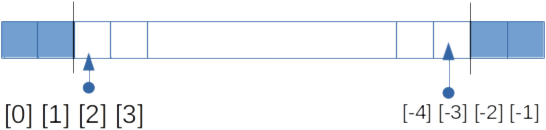
\includegraphics[scale=0.5]{./gridghost.png}
		\caption{Illustration of interior vs ghost zone}
	\end{figure}	
therefore, we see that if interior's indices run from -2 to 2, it includes all the white non-ghost cells since upper index--like python--is not included in the range.
	\item Primitive variable array \texttt{P} and magnetic field array \texttt{B} are both defined here as public variables which will be populated during the simulation.
	\item \texttt{void MeshData::applyBoundaryCondition (BoundaryCondition\& bc)} is also defined here, but it references the \texttt{BoundaryCondition::applySimple} method discussed in the next subsection.

\end{itemize}


\subsection{BoundaryConditions}
\begin{itemize}
	
	\item As previously mentioned in the Mara subsection, \texttt{void BoundaryCondition::applySimple (Cow::Array\& A, Cow::Shape boundaryShape) const} uses \texttt{apply} method to the left and right boundary on axis 0, 1 and 2 respectively. The \texttt{boundaryShape} array is supplied here which tells \texttt{Mara} how many ghostzones to include at each endpoint on the grid. This \texttt{applySimple} method is written such that it can take different flavors of \texttt{apply} methods corresponding to different derived classes. A few examples of them are \texttt{OutflowBoundaryCondition::apply}, or \texttt{ReflectingBoundaryCondition::apply}, each of which will override the virtual method stated in \texttt{Mara.h}. All the \texttt{apply} methods expectedly take identical arguments. We will analyze one of them in detail below for illustrative purposes.
	\item Let's look at the \texttt{PeriodicBoundaryCondition::apply}. Two things are defined within this method:
	\begin{enumerate}
		\item \texttt{auto guardZone = Cow::Region();}
		\item \texttt{auto validZone = Cow::Region();}
	\end{enumerate}
	They are both Region objects which describe specific regions within a multidimensional array. \texttt{guardZone} should be clear, whereas \texttt{validZone} describes the non-guardzone values within the mesh which determine the guardzone's values.
	\item Just looking at the \texttt{MeshBoundary::left} in the switch case, our intuition from matching periodic boundary conditions in solving wave equations or Schr$\ddot{\text{o}}$dinger's equation would tell us something like this: 
	
	\begin{figure}[H]
		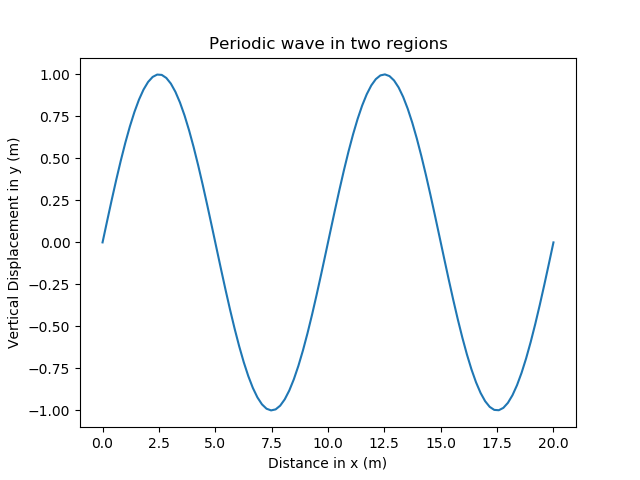
\includegraphics[scale=0.5]{./Wave.png}
		\caption{Periodic wave}
	\end{figure}
	
	Notice at x=0 and x=10, the wave repeats itself so to think of the periodic boundary condition, we can say $y(x=0)=y(x=10)$. Assume that now we're using 2 ghostcells to implement the BC. Refering back to Figure 1, it must mean that \texttt{A[0]=A[-4]} and \texttt{A[1]=A[-3]} at \texttt{MeshBoundary::Left}. Written more succinctly: \texttt{A[guardZone] = A[validZone];} where the guardzone is the array index range [0,1] and the validzone is the array index range [-4,-3]. 
	
	\item A brief note regarding the implementation of the reflecting boundary condition. Fluid behavior at a wall requires that the normal velocity: 
	\begin{equation}
		u_\perp=0.
	\end{equation}
Unfortunately, Dirichlet boundary conditions are not easily implemented using Finite-Volume Methods. However, the solution to that problem is to require that:
	$$\lim_{\Delta x \rightarrow 0}u(x-\Delta x) = -u(x+\Delta x) $$
	such that: 
	\begin{equation}
		u(x)|_{\partial\Omega} = -u(x)|_{\partial\Omega}
	\end{equation}
and the only solution is if $u(x) = 0$. One can treat $x-\Delta x$ as the first 2 ghostcells left of \texttt{MeshBoundary::Left} and $x+\Delta x$ as the first 2 validzone cells. In discrete form, that's equivalent to setting \texttt{A[1]=-A[2]} and \texttt{A[0]=-A[3]} on the \texttt{MeshBoundary::Left} in Fig 1.
	
	\item For completeness, the outflow boundary condition is simply to impose a zero-gradient condition at the boundary relative to the surface normal:
	\begin{equation}
		\mathbf{\hat{n}} \cdot \nabla \mathbf{u} = 0
	\end{equation}		
if we imagine a 1D grid like in Fig 1, eq. (3) is equivalent to saying:
	$$\frac{u_2^n-u_1^n}{\Delta x} = 0 \implies u_2^n = u_1^n$$.
	\item For example if we have 2 ghostcells, then outflow on \texttt{MeshBoundary::Left} would be equivalent to saying \texttt{A[0]=A[2]} and \texttt{A[1]=A[2]} as given by \texttt{void OutflowBoundaryCondition::apply}
	\item \texttt{MeshData} and this class are intricately linked since \texttt{MeshData::applyBoundaryCondition} method takes a \texttt{BoundaryCondition} object and uses the \texttt{applySimple} method. More on this in the MeshData subsection.
	
	
\end{itemize}

\subsection{ConservationLaws}
The \texttt{ConservationLaw.h} file contains different classes tailored to different conservation laws examined. A commonly used one is \texttt{class NewtonianHydro : public ConservationLaw} which you can tell inherits publicly from the parent \texttt{class ConservationLaw} from \texttt{Mara.h}. 

As you can see, this module provides specific implementation of the virtual methods defined in Mara's header file. Examples include \texttt{  int getNumConserved() const override;}, a function to get the number of conserved variables which would vary from 5 to 8 when one goes from Newtonian hydrodynamics to MHD. 
\begin{itemize}
\item Moving on to \texttt{ConservationLaw.cpp}, we see right off the bat, primitive names such as \texttt{\#define RHO 0} are set to an array index to facilitate data retrieval later. This is given a fancy name called fieldIndex. Be on the lookout for this in functions like \texttt{std::string NewtonianHydro::getPrimitiveName (int fieldIndex) const}.

\item Remember \texttt{Conservation::State} is defined in \texttt{Mara.h}, where it is a struct containing primitive/conserved arrays? It is used for example in \texttt{ConservationLaw::State NewtonianHydro::fromPrimitive (const Request\& request, const double* P) const}. 

\item The request (see \texttt{ConservationLaw::Request} defined in \texttt{Mara.h}) and a primitive array \texttt{P} are passed into the function. 

\item A \texttt{State S} is generated, and populated with primitives and conserved variables contained within the input array P. First off, we know mass density, 3 components of velocity and Pressure: $\rho$, $v_1$, $v_2$, $v_3$, $P$ comprise the primitive vector (5 component vector). Each one is given an index defined at the top of this file. This function takes these variables and generates conserved ones: $\rho \rightarrow \rho$, $v_1 \rightarrow	\rho v_1$. E.g. in the \texttt{.cpp} file, the \texttt{State S}'s momentum flux in direction 1: \texttt{S.U[S11] = P[RHO] * P[V11]}. Eigenvalues of the characteristics are also stored in this state. For Newtonian hydro, we know there are 3 distinct ones $\{v-c,v,v+c\}$, where c is the speed of sound.

\item An important function here are the diagnostic tools. One can use them to plot time series of mass, total energy to check the code's consistency. One example is the \texttt{ std::vector<double> NewtonianHydro::makeDiagnostics (const State\& state) const}, which you will need to pass a ConservationLaw::State in. The function creates an empty vector (of any size you want since it can contain as many diagnostics as you want), and it populates this vector with conserved variables.

The function is instrumental when trying to compute a time series of a volume-integrated variable. One thing of note is that this function represents the conserved variables within a particular cell, since volume-integrated quantities within a cell (defined as celld in \texttt{FieldOperator.cpp}):

$\texttt{diagnostics}=\int\limits_{\text{cell}} \left[\begin{smallmatrix}
	\rho \\
	\rho v_1 \\
	\rho v_2 \\
	\rho v_3 \\
	\frac{1}{2}\rho v^2 + \frac{P}{\gamma - 1}  
\end{smallmatrix} \right] dV$

 
\end{itemize}
 
\subsection{FieldOperator}
\begin{itemize}
	\item \texttt{FieldOperator} methods operate on the primitive/conserved variables. This module includes simple convenience functions like \texttt{getConservationLaw()} which returns a shared pointer to the conservation law used. 
	\item Other convenience functions include converting primitive variable arrays into conserved variables via \texttt{void generateConserved (Array::Reference P, Array::Reference U) const} which takes an array containing primitives P and puts the conserved variables into an empty array U. 
	\item One of the more important functions is getCourantTimeStep() and is computed here as well. \textbf{generateConserved(), getCourantTimeStep()}
	
	\item As mentioned in the previous subsection. An important diagnostic tool for sanity-checking the evolution of density-like thermodynamic quantities (i.e. entropy or total energy $e_T=e+\frac{1}{2}\rho v^2$, $e$ is the internal energy per unit volume) or momentum density in 3 dimensions $\rho \vec{v}$ in the Euler equations, is the \texttt{std::vector<double> volumeIntegratedDiagnostics (Array::Reference P, Array::Reference V) const} function. This returns volume integral (not volume average) of named diagnostics which are defaulted to `total\_energy' or 'mass' but one can customize this to ensure code is giving sensible results, \textbf{P and V contain primitives and cell volume for individual grid cells respectively throughout the whole mesh.} 
	\item \texttt{auto Treg = P.getRegion().withStride (3, law->getNumConserved())}. \texttt{Treg} is array P's region taking into account the stride. Recall that P is a 5 dimensional array, \texttt{withStride} here takes axes 3 (the number of components in a primitive vector) and sets that number to the number of conserved variables. This is to ensure we're getting the right primitive values.
	\item \texttt{Preg} is just the P array after taking into account the strided region of consideration.
	\item \texttt{pit} and \texttt{vit} represent pointer/iterators to these primitive vectors and cell volume of a particular cell; as the iterator is incremented by 1, we move to the next cell.
	\item  \texttt{celld = law->makeDiagnostics (state)} is what we described in the previous section and is a 5 component vector containing conserved variables at a particular cell location. 
	\item  This part: \texttt{diagnostics[n] += celld[n] * Vol} is looped over all the cells, hence summing the integrated to find the volume-integrated conserved variable of the whole mesh:
$$\text{Total diagnostic variable returned =} \sum_{\text{over mesh}} \texttt{diagnostics}$$
\end{itemize}

\subsection{MeshOperator}
\begin{itemize}
	\item Mesh operators are operators which Mara performs on the mesh grid itself (just spatial dimensions, doesn't touch primitive/conserved data in each cell). Common member functions include \texttt{divergence} and \texttt{curl}. One important one is \texttt{measure}, which returns the 1, 2, or 3 dimensional measure of the given mesh locations: length of edges, area of faces, or volume of cells.
	\item \texttt{Array MeshOperator::measure (MeshLocation location) const} can take \texttt{\{edge, face, cell\}}. Looking specifically at the \texttt{cell} switch case. \texttt{auto volumes=Array (geometry->cellsShape());} first creates a multidimensional array. 
	\item \texttt{Array::deploy (volumes.shape(), [\&] (int i, int j, int k)\{volumes (i, j, k)=geometry->cellVolume(i, j, k);\});} populates that aforementioned array with cell volumes corresponding to the individual index. As a reminder, \texttt{deploy} is a triple for-loop over the indices.
	\item \textbf{TALK ABOUT DIVERGENCE} 
	\item \textbf{AND GODUNOV METHODS HERE!!!!!}
	\item The core of generating a mesh is the function:
	\texttt{Array MeshOperator::generate (InitialDataFunction F, MeshLocation location, VectorMode vectorMode, Shape3D boundaryShape) const}. \texttt{totalCellsShape} is first defined and is set to the \texttt{cellsShape} (5 component array telling us how many gridcells in each dimension) taking into account ghostcells. So if \texttt{cellsShape = \{\{100,100,100,1,1\}\}}, \texttt{totalCellShape = \{\{104,104,104,1,1\}\}} if 2 ghostcells are present on each boundary.
	\item In particular, let's closely examine the switch case where \texttt{MeshLocation::cell} and not \texttt{face} or \texttt{edge}. Inside the block, \texttt{auto P = Array (totalCellsShape.withComponents (nq));}, this will become our primitive array. Additionally, \texttt{auto R = Region().withStride (3, nq);} makes sure the axes 3 contains \texttt{nq} number of primitive values (1 density + 3 momentum + 1 energy = 5 variables). 
	\item This means that \texttt{for (auto it=P[R].begin(); it!=P.end(); ++it) \{...\}} iterates over each cell in the mesh. For example, \texttt{int ic=it.index()[0]-boundaryShape[0]} gets the number of cells from the \underline{actual boundary of the mesh}. For instance, since there are 104 cells in the grid, first 2 being ghostcells, the first 2 validcells are labelled 2 and 3 in memory, but in fact should be labelled 0 and 1, corresponding to the physical location of the cells with respect to the grid.
	  
	\item \texttt{auto coord = geometry->coordinateAtIndex (ic, jc, kc)} simply picks out the physical coordinates (either in Cartesian (x,y,z) or spherical $(r,\theta,\phi)$). This is important since the \texttt{InitialDataFunction F} is passed these coordinates and is defined through \texttt{auto P0 = F (coord[0], coord[1], coord[2]);}.
	
	\item \texttt{it[q]=P0[q];}. Here, the program is looped through the individual primitives to set each cell with the initial primitive data.
	
	\item \texttt{Array MeshOperator::generateSourceTerms (SourceTermsFunction S, const Array\& P, Index start) const} has the basic design as the generate function. The analysis is left to the reader and is quite tractable.
	
\end{itemize}

\subsection{Scheduler}
\begin{itemize}
	\item Scheduler and logger are pointers that are passed through back into the maraMainLoop in the Mara.cpp file. Main function of scheduler is to put together a list of tasks to be completed at certain points when the code runs. They could include writing checkpoints or saving down time series data to ensure code is running properly and thereby optimizing data retrieval. An example of scheduler is \texttt{scheduler->schedule (taskTimeSeries, TaskScheduler::Recurrence (user["tsi"]), "time\_series");}. \texttt{taskTimeSeries} is a callback lambda which the function takes as input, thereby telling the scheduler what function to use to perform a specific task at certain periods of time during runtime. What determines \emph{when} the task is performed depends solely on the \textbf{recurrence rule}. This literally means, when will the task/function recurr in the program via some hard and fast rule. In this case, \texttt{TaskScheduler::Recurrence (user["tsi"])} does just that using \texttt{user["tsi"]} which is specified at runtime. \textbf{SPLIT LOGGER INTO SEPARATE PARAGRAPH}
\end{itemize}


\subsection{Problems}
This is a section 

\subsection{RiemannSolvers}
This is a section 

\subsection{IntercellFluxSchemes}
Tie this in with SolutionSchemes and RiemannSolvers

\subsection{SolutionSchemes}
\begin{itemize}
	\item \texttt{SolutionSchemes} contain the main tool used for evolving the initial data. This module is dependent on IntercellFluxScheme and the RiemannSolver module mainly in order to advance the solution. 
	\item \texttt{void MethodOfLinesTVD::advance (MeshData\& solution, double dt) const} is the core method of advancing the solution forward in time. 
	\item To get a feel for how this method works, we first review what the algorithm is doing: 
	$$\frac{\partial \mathbf{U}(\mathbf{x},t)}{\partial t} + \nabla \cdot  \mathbf{F}(\mathbf{x},t) = \mathbf{S}$$ where $\mathbf{U}$ is the conserved vector and $\mathbf{F}$ is the conserved flux vector. Using the method of lines, we discretize this PDE in space while keeping ODE's in time. Just writing out the discretized version of this equation for cell $j$ (cell average) after performing an $\int dV$ and converting $\nabla \cdot \mathbf{F}$ into a surface integral:
	\begin{equation}
	\frac{d \mathbf{U_j}(t)}{dt} = \mathbf{S}_{j}(t)- \sum_{\text{all faces}} \text{Area} \cdot \text{Flux}
	\end{equation}
where we multiply each cell face area by the flux vector through that face. If we now discretize LHS in time using Runge-Kutta, we recover how \texttt{advance} function works.
	\item \texttt{auto F = meshOperator->godunov (Fhat, solution.P, solution.B, footprint, startIndex, fieldCT);} is the computed Godunov flux through the cell interfaces. Details in FieldOperator subsection above.
	\item \texttt{auto Fhat = [\&] (GodunovStencil\& stencil)} is the lambda responsible for using a Riemann Solver to resolve the intercell fluxes. Hence, the cell face data is required here.
	\item \texttt{auto L = meshOperator->divergence (F, -1.0);} is the divergence (surface integral mentioned above) multiplied by $-1$.
	\item \texttt{auto S = meshOperator->generateSourceTerms (sourceTermsFunction, solution.P, startIndex);} is denoted as $\mathbf{S}_j$ above. 
	\item \texttt{L[n] += S[n];} is looped over all gridcells and just represents RHS in eq. (4)
	\item \texttt{U[n]=U0[n]*(1-b[rk])+(U[n]+dt*L[n])*b[rk];} is just the RK implementation for the timestep integration.
	\item And this last part is for generating the primitives again from the conserved and storing it in memory: \texttt{fieldOperator->recoverPrimitive (U[interior], solution.P[interior])}
\end{itemize}








\end{document}